\chapter{Introduction to Wireless Sensor Networks} \label{chap:IntroWSN}
This chapter presents a brief introduction to Wireless Sensor Networks (WSNs).
Additionally, it describes the reference WSN protocol stack used as part of this
work, and provides a short overview of WSN routing techniques.

\section{Sensor Nodes} \label{subsec:sensornodes}
WSNs are, as described earlier (see Chapter \ref{chap:Intro}), networks of sensor
nodes, and are typically deployed randomly in a possibly large area where
phenomena are required to be monitored.

As presented in Figure \ref{Fig:SensorNodeArch}, a sensor node consists of
the following elements:
\begin{itemize}
  \item \emph{Sensing unit}, which is comprised of a number of sensors and
  analog-to-digital converters. 
  \item \emph{Transceiver}, which facilitates node-node communication using 
a variety of techniques.
  \item \emph{Processing unit}, that comprises a 
microcontroller/microprocessor that performs processing, and is associated with 
a storage unit.
  \item \emph{Power unit}, which provides the energy required to run the sensor node, and can use chemical 
batteries or power scavenging units such as solar cells.
\end{itemize}

\begin{figure}[h]
\centering
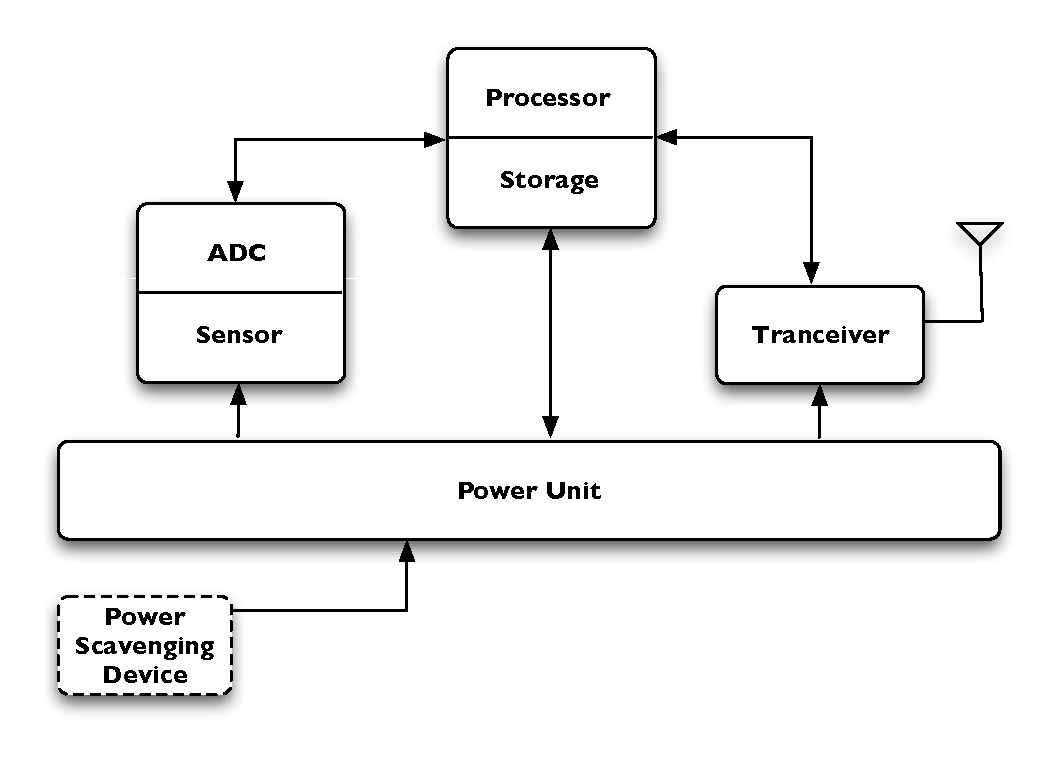
\includegraphics[scale=0.65]{img/SensorNodeArch.eps} 
\caption[Architecture of a sensor node] {Architecture of a sensor node (adapted from \cite{SensorSurveyAkyildiz:2002}).}
\label{Fig:SensorNodeArch}
\end{figure} 

Due to the small size of the devices, sensor nodes have a number of constraints
which affect the WSN built on top of it. These include \cite{yao:qps}:
\begin{itemize}
  \item \emph{Power consumption constraint,} due to the fact that sensor nodes
  have limited energy supply. Therefore, energy conservation is the main concern when
  WSN applications are implemented.
  \item \emph{Computation restriction,} caused by the limited memory
  capacity and processing power available on the sensor node. This places
  serious limitations on the use of data processing algorithms on a sensor node.
  
  \item \emph{Communication constraint,} as a result of the minimal bandwidth available and a
  limited Quality of Service (QoS) provided by the sensor node's hardware. 
\end{itemize}

Additionally, as the deployment of sensor nodes in the WSNs should be
cost-effective, the cost of a single device is a supplementary constraint.

A WSN is self-organising system, given the random nature of the deployment. Its
topology is subject to change because of characteristics of the wireless medium,
and therefore, sensor nodes should be capable of dealing with changes of this kind in order to cope with hostile operating
conditions, the failure-prone nature of sensor nodes and the possibility of
redeployment of additional sensor nodes at any time during operation.

\section{WSN Protocol Stack} \label{sec:WSNProtStack}

The WSN protocol stack presented in \cite{SensorSurveyAkyildiz:2002} is an
adaptation of a generic protocol stack \cite{ComputerNetworksTannenbaum:2003}.


\begin{figure}[h]
\centering
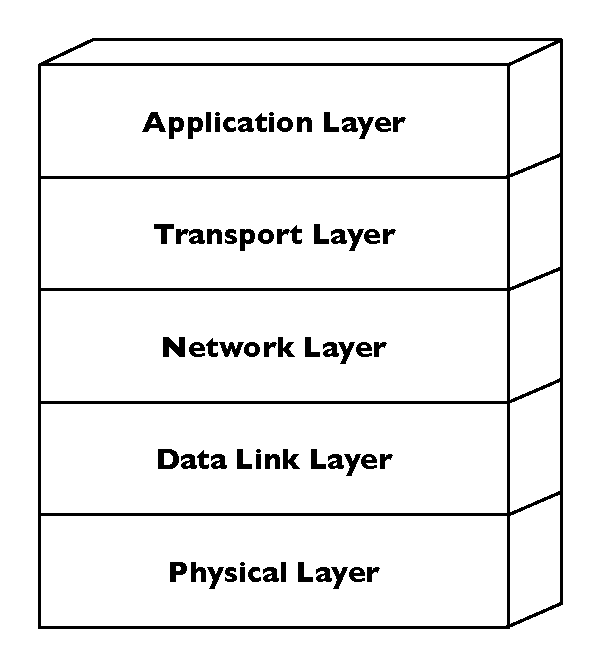
\includegraphics[scale=0.65]{img/ProtStack.eps}
\caption[WSN protocol stack]{WSN protocol stack (reproduced from \cite{SensorSurveyAkyildiz:2002})}
\label{Fig:ProtStack}
\end{figure}

According to \cite{SensorSurveyAkyildiz:2002} the WSN protocol stack consists
of the following layers:

\begin{itemize}
\item \emph{Physical Layer}, which provides the transmission of data over the physical transmission medium.
\item \emph{Data Link Layer}, which deals with power-aware Medium Access Control (MAC) protocols that minimise collisions and transceiver on-time.
\item \emph{Network Layer}, which is primarily responsible for
routing data across the network.
\item \emph{Transport Layer}, which provides reliable delivering of data and
supports error checking mechanisms.
\item \emph{Application Layer}, where the application software resides.
\end{itemize}

The work presented here is resided fully on the application layer of the
protocol stack, but uses network layer .. . %%%% TO WRITE UP (TO COVER WHY WE
%DECRIBE PROTOCOL STACK )

%\section {Routing in WSNs}

%The existing constraints of the sensor nodes influence the design of routing
%protocols, and these limitations have to be overcome in order to provide
%efficient communication in WSNs \cite{routing:2004}.

%Routing algorithms may be classified on the basis of the organisation of
%the network structure used. Routing algorithms are thus primarily classified
%into being either:
%\begin{itemize}
%\item \emph{Flat}, where every node plays the same role, 
%\item \emph{Hierarchical}, where the network is organised into physically
%defined clusters,
%\item \emph{Location-based}, where positioning information is used to direct
%traffic to a given physical subset of the network.
%\end{itemize}

%Additionally, depending on how the source finds a route to the destination
%routing protocols can be split into three categories \cite{routing:2004}:
%\begin{itemize}
%	\item \emph{Proactive}, when all routes are known before they are used
%	\item \emph{Reactive}, when route is computed on demand 
%	\item \emph{Hybrid}, which uses a combination of the two techniques above.
%\end{itemize}

%The LN routing algorithm that is principal to this work may be considered as an
%exaple of a hybrid routing algorithm, as logical predicates
%are used to direct traffic to a specific \emph{logical} subset of the network.
%A more detailed discussion of the LN mechanism may be found in
%Chapter \ref{chap:background}.

\section {Programming Models for WSNs}

Current WSN programming paradigms are predominantly node-centric, wherein
applications are monolithic and tightly coupled with the protocols and algorithms
used in the lower layers of the protocol stack. 
The main reason for this is the limited resources available on the sensor node, as
was previously discussed in Section \ref{subsec:sensornodes}.

The primary problem with a node-centric approach is that most WSN applications
are developed at an extremely low level of abstraction, which requires the programmer to be knowledgeable in the field of
embedded systems programming. This stunts the growth in the use of WSNs in the
large space of application domains where it may potentially be of use
\cite{mottola_middleware:2008}. 

To increase the ubiquity of WSN
usage, it is essential that protocols and mechanisms underlying WSN
development recede to the background, and the application programmer is
empowered to develop WSN applications at a higher level of abstraction. This
can be achieved using programming models that engineer a shift in focus
towards the system and its results, as opposed to sensor node functionality
itself \cite{mottola_middleware:2008}. 

According to Yu et al \cite{yu_issuesMiddleware:2004}, the use of such
programming models is beneficial for WSN applications because:
\begin{itemize}
\item The semantics of a WSN application can be separated from the details of 
the network communication protocol, OS implementation and hardware.
\item Efficient programming models may facilitate better utilisation of system 
resources.
\item They facilitate the reuse of WSN application code.
\item They provide support for the coordination of multiple WSN applications.
\end{itemize}

\subsection{Taxonomy of WSN Programming Models}

\begin{figure}
\centering
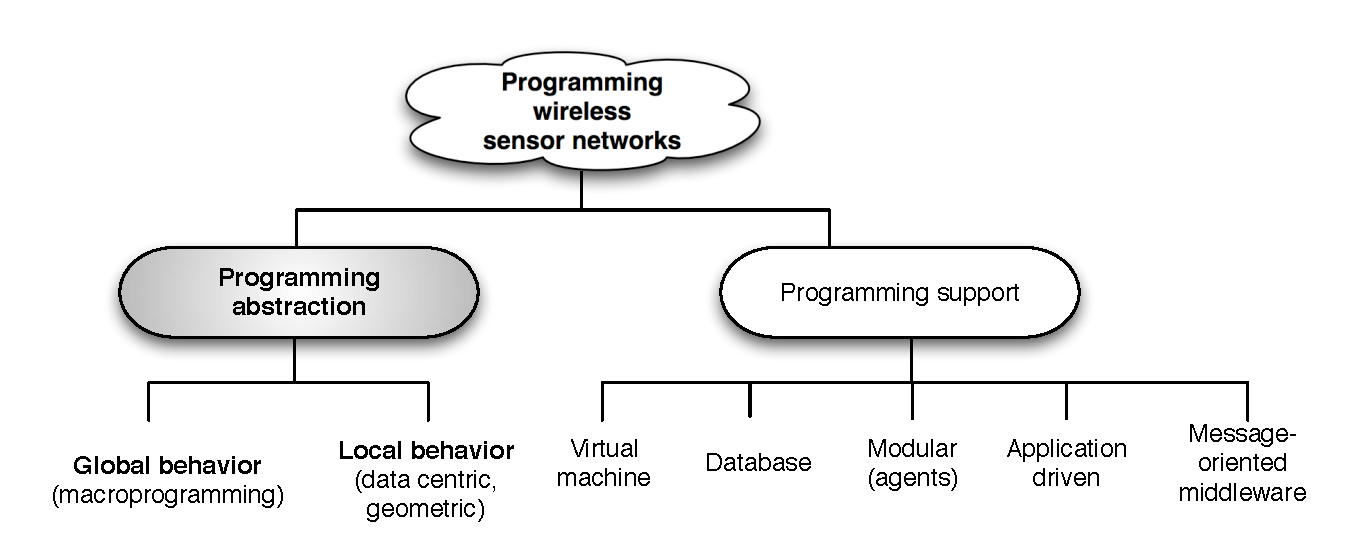
\includegraphics[width=\textwidth]{img/ProgrammingAbstractions.eps} 
\caption[Taxonomy of WSN programming models]{Taxonomy of WSN programming models (reproduced from
\cite{hadim_middleware:2006})}
\label{Fig:ProgrammingModels}
\end{figure}

Existing programming models for WSNs cover different areas and can serve 
several different purposes. They can be classified into two main types, depending on 
the applications they are used for  \cite{hadim_middleware:2006} (see Figure
\ref{Fig:ProgrammingModels}):
\begin{itemize}
\item \emph{Programming support}, wherein services and mechanisms allowing for 
reliable code distribution, safe code execution, etc. are provided. Some
examples of programming models that take this approach include Mate
\cite{Levis_Mate:2002}, Cougar \cite{Bonnet_Cougar:2001}, SOS
\cite{Han_SOS:2005}, and Agilla \cite{Fok_Agilla:2005}.
\item \emph{Programming abstractions}, where models deal with the global view 
of the WSN application as a system, and represent it through the concepts and 
abstractions of sensor nodes and sensor data. Some
examples of programming models that take this approach include Kairos \cite{gummadi_Kairos:2005}, and
EnviroTrack \cite{Abdelzaher_EnviroTrack:2004}.
\end{itemize}

This section further discusses and classifies a subset of WSN programming
models, namely WSN programming abstractions.

Programming abstractions may be distinguished depending on the way WSN nodes
are being programmed, and therefore either be
\emph{global} (also referred to as macroprogramming) or \emph{local} \cite{hadim_middleware:2006}. 

In the former case, the sensor network is programmed as a whole, and gets rid of
the notion of individual nodes \cite{mottola_middleware:2008}. Examples of
macroprogramming solutions include \emph{TinyDB} \cite{madden_TinyDB:2005} and
\emph{Kairos} \cite{gummadi_Kairos:2005}. 

In the latter case, the focus is on identifying relevant sections or
\emph{neighbourhoods} of the network. It is to be noted that these neighbourhoods
need not necessarily be physical. The framework used and developed during the
course of this work belongs to the latter class of programming abstractions.

Programming abstractions may also be classified on the basis of the
nature of the language constructs made available to the WSN programmer
\cite{mottola_middleware:2008}. 

Classification of WSN programming abstractions w.r.t. language constructs is
presented in Figure \ref{Fig:ProgrAbstrClassification}.

\begin{figure}
\centering
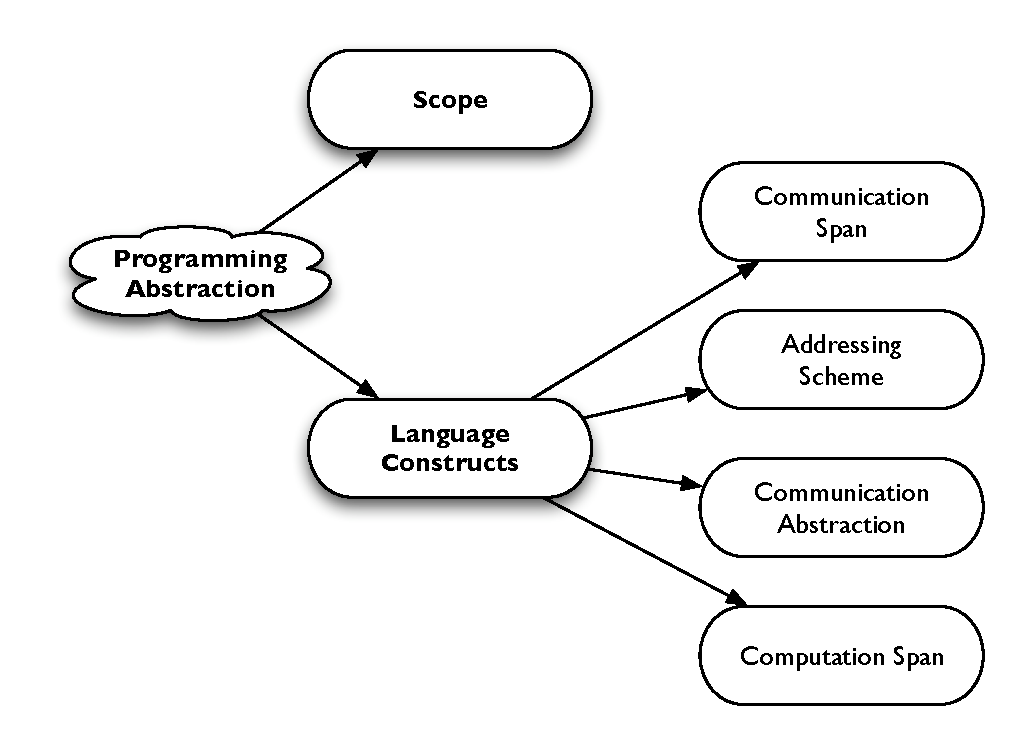
\includegraphics[scale=0.65]{img/ProgAbstr_Classification.eps}
\caption{Classification of Programming Abstractions (adapted from \cite{mottola_middleware:2008})} 
\label{Fig:ProgrAbstrClassification}
\end{figure} 

The rest of this section discusses each of these bases for classification in
detail, and is based on the work described in \cite{mottola_middleware:2008}
unless explicitly mentioned otherwise.

\subsubsection{Communication Span}

The \emph{Communication span} enabled by a WSN programming interface is defined
as the set of nodes that communicate with one another in order to accomplish a
task. The communication span provided by a given abstraction can be
\cite{mottola_middleware:2008}:
\begin{itemize}
  \item \emph{Physical neighbourhood}
  \item \emph{Multi-hop group}
  \item \emph{System-wide}
\end{itemize}

Abstractions that use \emph{physical neighbourhood} approach provide
  the programmer with constructs to allow nodes to exchange data with others
  within direct communication range. Examples of communication in physical
  neighbourhood include nesC \cite{nesc:2003} and Active Messages \cite{activemessagesEicken:2001}.
  
Abstractions with \emph{multi-hop group} approach allow the
  programmer to exchange data among subsets of nodes in the WSN using
  multi-hop communication. These sets may either be
  \emph{connected}, wherein there always exists a path between any two nodes in
  the set, or \emph{non-connected/disconnected}, where ``no assumptions on the geographical location of nodes 
belonging to the group'' \cite{mottola_middleware:2008} can be made.  
  EnviroSuite Framework \cite{envirosuite:2006} represents an example of
  connected multi-hop communication, and Logical Neighborhoods
  \cite{mottola_LN:2006} - an example of non-connected multi-hop
  communication.

\emph{System-wide} abstractions let the
  programmer use constructs that allow data exchange between any two nodes
  of the entire WSN. This may be seen as an extreme manifestation of the
  \emph{multi-hop group} approach mentioned above. An example of system-wide
  communication is TinyDB \cite{madden_TinyDB:2005} project.
  
\subsubsection{Addressing Scheme}

The \emph{addressing scheme} specifies the mechanism by which nodes are
identified. Typically, there are two kinds of addressing schemes used
\cite{mottola_middleware:2008}:

\begin{itemize}
  \item \emph{Physical addressing}
  \item \emph{Logical addressing}
\end{itemize}

In \emph{physical addressing} schemes nodes are identified using unique 
  identifiers. The same address always identifies the same node (or nodes, if
  duplicate  identifiers exist) at any time during the execution of the
  application. The paradigmatic example of physical addressing scheme is Active
  Messages communication \cite{activemessagesEicken:2001}.

When a \emph{logical addressing} mechanism is used, nodes are identified on the
basis of application-level properties specified by the application
programmer. Therefore, the same address, i.e. set of
application-level predicates, can identify different sets of nodes at different
times. An example of logical addressing is Logical Neighborhood communication
\cite{mottola_LN:2006}.

\subsubsection{Communication Abstraction}

This classification basis defines the degree to which details of communication
in a WSN are hidden from the application programmer's view. Programming
interfaces may provide either \cite{mottola_middleware:2008}:
\begin{itemize}
  \item \emph{Explicit communication} primitives where the
  programmer working in the application layer has to handle communication
  aspects such as buffering and parsing. 
  \item \emph{Implicit communication}, where the programmer is unaware of the
  details of the communication process, and communicates using
  high-level constructs.
\end{itemize}

Active Messages \cite{activemessagesEicken:2001} present an example of
explicit communication approach. In contrast, the Active Regions programming
framework \cite{activeregions:2004} belongs to the latter category.

\subsubsection{Computation Span}

The \emph{Computation span} enabled by a WSN programming interface is defined
as the set of nodes that can be affected by the execution of a single
instruction. The
computation span provided by a given abstraction can be
\cite{mottola_middleware:2008}:

\begin{itemize}
  \item \emph{Node}, when the effect of any instruction is restricted to a
  single node.
  \item \emph{Group}, where the programmer is provided with constructs that
  could affect a subset of nodes. 
  \item \emph{Global} present an extreme case of previous type, a single
  instruction can impact every node in the WSN.
\end{itemize}

An example of node computation is the ATaG framework \cite{atag:2005}; the
Regiment system \cite{regiment:2007} implements group communication approach. The
TinyDB \cite{madden_TinyDB:2005} represents an example of global computation
span.

\subsection{Programming Models on the WSN Protocol Stack}

\begin{figure}
\centering
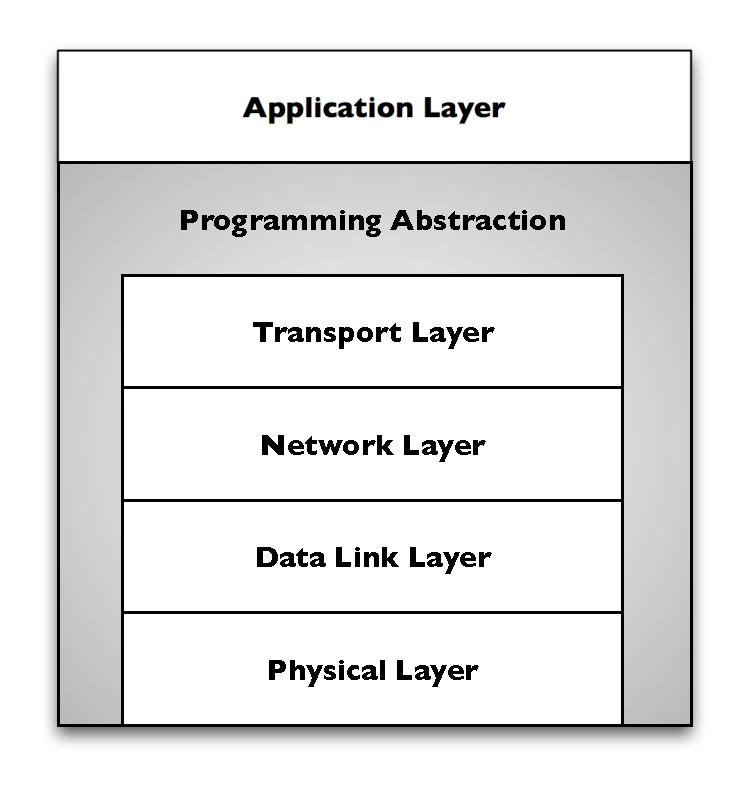
\includegraphics[scale=0.61]{img/ProtStack_ProgAbstr.eps}
\caption[Programming models on the WSN protocol stack]{Programming models on the WSN protocol
stack (adapted from \cite{mottola_middleware:2008})}
\label{Fig:ProtStack_ProgAbstr}
\end{figure}

WSN programming models often are placed between the application layer and the
transport layer in the protocol stack shown in Section \ref{sec:WSNProtStack}. As it can be seen from
Figure \ref{Fig:ProtStack_ProgAbstr},
fine-grained details are hidden from the application programmer's view. These
include:

\begin{itemize}
  \item Higher-layer services such as routing, localisation, and data storage
  mechanisms (and optimisations).
  \item Lower-layers such as the MAC protocol used, and the physical means of
  communication such as RF communication.
\end{itemize}

\section{Summary}
This chapter presented an introduction to WSNs and discussed in detail the 
sensor nodes that constitute them. This was followed by a description of the WSN
protocol stack. The chapter concluded with a classification of
existing WSN routing mechanisms, and placed the techniques and concepts used during the course of
this work within this classification.


